\documentclass[10pt,a4paper]{article}

% Modern font setup
\usepackage{fontspec}
\usepackage{unicode-math}

% Font selection
\setmainfont{Fira Sans}
\setsansfont{Fira Sans}
\setmonofont{Fira Code}
\setmathfont{Fira Math}

% Language and layout
\usepackage[utf8]{inputenc} % optional with XeLaTeX, but safe
\usepackage[brazil]{babel}
\usepackage{geometry}
\geometry{margin=2.5cm}

% Good to keep
\usepackage{amsmath}
\usepackage{graphicx}
\usepackage{url}
\usepackage{xcolor}
\usepackage{outlines}

% Bibliography
\usepackage[backend=biber,style=authoryear]{biblatex}
\addbibresource{references.bib}
\renewcommand*{\nameyeardelim}{\addcomma\space}

\title{Estruturação de Estados\\ orientada a Game Design\\ em Aprendizado por Reforço}
\author{{\bfseries Marcelo Augusto Salomão Ganem }\\ Universidade Federal de Minas Gerais\\
\texttt{marceloganem@dcc.ufmg.br}
}
\date{\today}

\newcommand{\note}[1]{
    \vspace{0.3cm}
    \colorbox{blue!30}{
            \begin{minipage}{0.4\textwidth}
		    \ttfamily \footnotesize
               #1
            \end{minipage}
        }
    \vspace{0.3cm}
}

\setlength{\columnsep}{1cm} % or whatever you prefer
\begin{document}

\makeatletter
\begin{titlepage}
  \centering
  \vspace*{5.5cm}
    {\Large \bfseries Proposta de Pesquisa Científica - MSI I \par}
    \vspace{1cm}
    {\Huge \bfseries \@title \par}
  \vspace{1cm}
  \vspace{0.5cm}
    {\bfseries Aluno\par}
  {\Large \@author \par}
  \vspace{0.5cm}
    {\bfseries Orientador\par}
  {\Large {\bfseries Prof. Luiz Chaimowicz }\\ Universidade Federal de Minas Gerais\\\texttt{chaimo@dcc.ufmg.br} \par}

  \vfill {\large \today\par}
\end{titlepage}

\twocolumn
\begin{abstract}
    A escolha de estados representativos em tarefas de aprendizado por reforço é essencial na construção de modelos com comportamentos explicáveis e previsíveis. Essa Proposta de MSI tem por pretensão investigar a qualidade de modelagens de Processos de Decisão de Markov orientadas a aspectos bem-definidos de \textit{game design} na implementação de agentes de IA para jogos. Como justificativa e orientação para a pesquisa, as literaturas de inteligência artificial, aprendizado por reforço e design de jogos servem a base para a construção de modelos coerentes dos problemas comumente enfrentados em jogos.
\end{abstract}


\label{introduction}
\section{Introdução}

Agentes de aprendizado por reforço aprendem e interagem com o mundo por meio de abstrações de ambientes reais. Para o caso particular de jogos, eletrônicos ou não, é frequente a necessidade de modelar mecânicas simples que interagem entre si para produzir comportamentos complexos.

\label{topic}
\subsection{Tópico da pesquisa}

A tarefa de modelar jogos a partir da definição de suas mecânicas de maneira formal foi inicialmente explorada por \citeauthor{machinations} (\citeyear{machinations}), mas ainda não integrada a estratégias de aprendizado de máquina, no geral, ou de aprendizado por reforço, que é o escopo específico do presente trabalho.

Investigamos, portanto, a aplicabilidade de tais modelagens desenvolvidas a partir de regras estritas (ver Seção \ref{references:machinations}) na construção de modelos de aprendizado por reforço capazes de responder coerentemente às estruturas\footnote{Estruturas lógicas referentes à economia de recursos e condições de vitória.} de jogos -- idealmente, de maneira generalizada.

\subsection{Relevância}
\label{relevance}

As perguntas aqui propostas são caminhos para avançar o conhecimento em aprendizado por reforço, especificamente no domínio da interpretabilidade por meio de modelagens bem estruturadas. Entende-se uma representação de estado em \textit{features} que correspondam a aspectos explicitamente definidos do ambiente como uma ferramenta para produzir agentes cujo comportamento pode ser mais coerentemente explicado.

Ainda, tais questões são relevantes para o desenvolvimento de inteligência artificial em jogos de uma maneira geral. Partindo de um referencial centrado em \textit{game design} -- evitando, portanto, miopias particulares de uma perspectiva estritamente computacional, espera-se que o método aqui executado seja replicável na indústria de jogos eletrônicos em geral, bem como na otimização de mecânicas em jogos de tabuleiro.

\subsection{Objetivos}
\label{goals}

O escopo do trabalho é divido em dois semestres, correspondentes às disciplinas MSI I e II. Assim, definimos os objetivos da \textbf{MSI I} como:

\begin{outline}

	\1\textbf{Objetivo geral}:
	\2 Responder a \textit{research question}: "Qual é o impacto de providenciar uma representação de estado estruturada para agentes de aprendizado por reforço na convergência e captura de padrões complexos em jogos?"

	\1\textbf{Objetivos específicos}:
	 \2 Implementar simulações de diagramas \textit{Machinations} em código aberto\footnote{Disponíveis à época da publicação, hoje são propriedade intelectual da empresa de mesmo nome. O trabalho orginal, entretanto, está sob a \textit{Creative Commons License}.};
	 \2 Treinar agentes de aprendizado por reforço via Q-Learning e DQNs, utilizando um modelo observacional estruturado com base em grafos de \textit{Machinations}.
	 \2 Investigar a performance e convergência dos modelos desenvolvidos.

\end{outline}

Observa-se que a expectativa não é contemplar todos os detalhes da sintaxe proposta por \citeauthor{machinations}. Para a \textbf{MSI 2}, pretende-se:

\begin{outline}
	\1 \textbf{Objetivo geral}:
    \2 Responder a \textit{research question}: "A utilização de \textit{Graph Neural Networks} em combinação com representações de estado estruturadas pode auxiliar na generalização do aprendizado de padrões em jogos?"
	
	\1 \textbf{Objetivos específicos}:
	\2 Implementar GNNs capazes de processar o estado do ambiente formatado como um grafo.
	\2 Processar definições de jogos na sintaxe \textit{Machinations} com entradas de tamanho variável.
    \2 Aferir a capacidade de generalização de modelos de \textit{Deep Reinforcement Learning} que interpretem diagramas \textit{Machinations} diretamente como grafos.

\end{outline}

\section{Referencial Teórico}
\label{references}

\subsection{Engineering Emergence}
\label{references:machinations}
A sintaxe \textit{Machinations} \parencite{machinations} é introduzida por \citeauthor{machinations} como parte da sua tese de doutorado "\textit{Engineering Emergence: Applied Theory for Game Design}". Seu elemento central é a definição de uma gramática de elementos para a composição de um grafo cuja premissa é representar o estado da economia interna de um jogo.
\begin{figure}[h!]
    \centering
    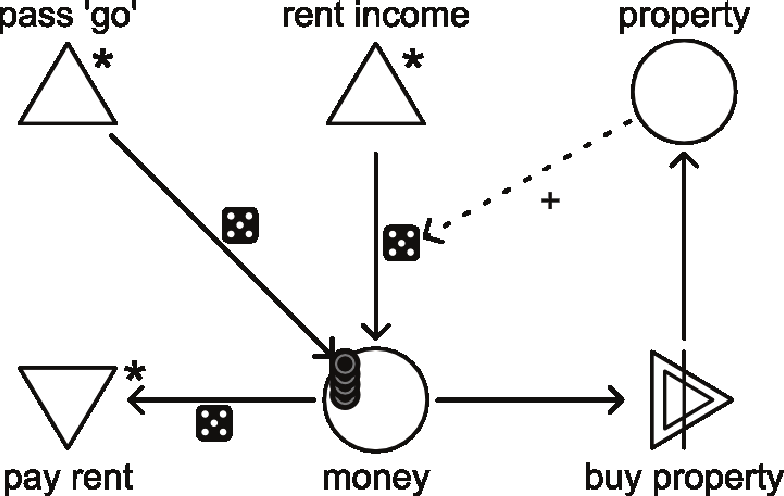
\includegraphics[width=0.9\linewidth]{figures/monopoly.png}
    \caption{Representação do jogo \textit{Monopoly} (\citeyear{monopoly}) sob a sintaxe \textit{Machinations}}.
    \label{fig:monopoly}
\end{figure}

\citeauthor{machinations} define essa economia interna como a alocação dos recursos (representados na Figura \ref{fig:monopoly} como fichas em cima de cada nó) entre os nós. O estado dessa economia é alterado a partir do andamento discreto do tempo e ações do jogador ou de quaisquer agentes presentes no sistema. O caráter dessas transições, i.e., o estado atingido em seguida, é ditado pelas arestas do grafo, que indicam transferência regular, condicional ou probabilística de recursos.

\subsection{Reinforcement Learning}
\label{references:rl}
O modelo proposto por \citeauthor{machinations} é análogo em vários aspectos a um Processo de Decisão de Markov (MPD), como introduzido por \citeauthor{rl}  -- que não inventaram o conceito, mas cuja literatura serve como referência para essa e outras definições fundamentais no contexto de aprendizado por reforço \parencite{rl}.


Em um MDP, temos um agente que interage com um ambiente cujo estado se altera com o tempo e com as ações desse agente -- ou de outros agentes, em alguns casos. O objetivo é maximizar a recompensa recebida para cada um dos estados atingidos a partir das ações tomadas. Semelhantemente, em um jogo modelado na sintaxe \textit{Machinations}, o objetivo é direcionar a economia interna para um estado terminal onde o jogador vença o jogo ou continuamente estabeleça uma economia favorável a si.

Assumindo que a economia interna de um jogo possua a \textit{Markov property}, i.e., que seus estados possam ser inferidos sequencialmente sem dependência de qualquer estado além do antecessor, podemos aplicar a maioria das técnicas introduzidas por \citeauthor{rl} em "\textit{Reinforcement Learning: An Introduction}". Naturalmente, recorre-se à aproximação em casos práticos -- assim, desde que o estado possa ser razoavelmente inferido sob o modelo de um MDP, o escopo de estratégias de \textit{Reinforcement Learning} ainda se aplica.

\subsection{Artificial Intelligence: a modern approach}
Um diagrama na sintaxe \textit{Machinations} também revela informação pertinente ás principais taxonomias para desafios em inteligência artificial propostas por \citeauthor{ai} (\citeyear{ai}). Uma análise estática do tipo de cada um dos nós e arestas do grafo revela se o ambiente a ser modelado é determinístico ou estocástico, diferenciando inclusive ambientes estacionários de não-estacionários. Semelhantemente, essa análise revela se o ambiente inclui outros agentes, se a interação é competitiva ou colaborativa e se o ambiente é episódico ou sequencial.

Apesar de sua implementação ser adequada para \textit{estados} contínuos, \citeauthor{machinations} decide não cobrir o caso de \textit{ambientes} denominados contínuos sob a definição de \citeauthor{ai}. Isso se deve à limitação do trabalho à análise de mecânicas e dinâmicas discretamente representáveis em jogos -- que se estende para essa MSI.

\section{Metodologia}
\label{methodology}

Propõe-se responder as perguntas introduzidas na Seção \ref{goals} pela construção de representações de estado em cenários de Aprendizado de Reforço que capturem as informações contidas em um diagrama de \textit{Machinations}. A qualidade dessas representações, mensurada a partir da performance do agente, informa a efetividade da modelagem proposta.

\subsection{Simulação da sintaxe \textit{Machinations}}

As definições em \textit{Engineering Emergence} permitem a simulação dos diagramas como uma máquina de estado cujos comportamentos são determinados pelos tipos de arestas, tipos de nós e conexões entre eles. Semelhantemente, pode-se implementar o modelo proposto como um MDP que se altera com a passagem do tempo em intervalos discretos.

Essa etapa consiste de implementar as funcionalidades de diagramas \textit{Machinations}, tal que o estado -- i.e., o alocamento dos recursos entre os nós -- se altere apropriadamente a partir de ações e tempo conforme as definições da sintaxe.
% \note{
	%Desenvolver modelos para os grafos. Os nós devem ter tipos, arestas também.  Podemos trabalhar com herança e composição aqui -> conversor é uma composição, mas uma pool é uma herança, sei lá. Rever o livro. Podemos focar esse desenvolvimento na ideia de aplicar GNNs.
%}

\subsection{Modelagem de jogos sob a sintaxe \textit{Machinations}}

Com diagramas que podem ser consistentemente simulados, a etapa seguinte é modelar jogos como grafos na sintaxe definida -- esse será o ambiente onde os agentes serão efetivamente treinados. Jogos comuns e amplamente discutidos na obra de referência são 
\textit{Monopoly} (\citeyear{monopoly}) e \textit{Settlers of Catan} (\citeyear{catan}). A coleção de jogos implementados deve ser representativa da diversidade de ambientes com os quais se espera que os agentes sejam capazes de lidar.

 \subsection{\textit{Baselines}}
 Para comparação, são necessários modelos de aprendizado por reforço que não utilizem representações estruturadas de estado. Assim, essa etapa contempla a implementação de um agente de \textit{Q-Learning} e um agente baseado em \textit{Deep-Q Networks} que sejam \textit{naïve} com relação à estrutura do estado.

 \subsection{\textit{Informed Q-Learning Agents}}
O primeiro experimento implementa agentes de \textit{Q-Learning} que recebem o estado como uma entrada estruturadas. Nós e seus tipos, bem como arestas e seus tipos, serão representadas como \textit{features} para o modelo. Essa solução relativamente simples deve permitir aferir com clareza as implicações da estrutura proposta para o estado.

\subsection{\textit{Deep-Q Networks}}
Expandir as soluções de \textit{Q-Learning} com técnicas de Aprendizado Profundo. A expectativa é que soluções como DQNs sejam capazes de capturar padrões mais complexos como \textit{feedback loops}, múltiplas condições de vitória e aspectos específicos a cada jogo. A exploração de outras técnicas de Aprendizado Profundo faz parte do escopo da MSI II, para o semestre seguinte.

\section{Resultados Esperados}
\label{expected-results}

Espera-se, especialmente, que agentes de aprendizado por reforço treinados a partir da modelagem \textit{Machinations} de um jogo sejam capazes de identificar estratégias ótimas e condições de vitória para cada jogo analisado. Ainda, com a adoção de técnicas de aprendizado profundo, espera-se que os aprendizados dos modelos sejam generalizados para jogos modelados sob a mesma sintaxe. Tais aspectos qualitativos serão inferidos a partir de métricas que incluem número de episódios até a convergência, taxa de vitória, recompensa média por episódio e recompensa acumulada, analisados comparativamente com o auxílio de visualizações.
\section{Etapas e Cronograma}
\label{plan}

\textbf{Semana 1 (22/04 -- 28/04):} Definição da metodologia, alinhamento da proposta e levantamento preliminar da literatura.

\vspace{0.5em} % espaço entre os parágrafos

\textbf{Semana 2 (29/04 -- 05/05):} Revisão de literatura e estudo detalhado dos diagramas \textit{Machinations}.

\vspace{0.5em}

\textbf{Semana 3 (06/05 -- 12/05):} Início da implementação da simulação da sintaxe \textit{Machinations} e desenvolvimento do modelo de máquina de estados.

\vspace{0.5em}

\textbf{Semana 4 (13/05 -- 19/05):} Continuação da implementação, realização de testes preliminares e ajustes na simulação.

\vspace{0.5em}

\textbf{Semana 5 (20/05 -- 26/05):} Modelagem dos jogos (por exemplo, \textit{Monopoly} e \textit{Settlers of Catan}) conforme a sintaxe proposta e integração ao ambiente de simulação.

\vspace{0.5em}

\textbf{Semana 6 (27/05 -- 02/06):} Desenvolvimento dos agentes de \textit{Q-Learning} utilizando a representação de estado estruturada.

\vspace{0.5em}

\textbf{Semana 7 (03/06 -- 09/06):} Testes e ajustes dos agentes de \textit{Q-Learning}; preparação para o primeiro pitch (previsto para 06/06).

\vspace{0.5em}

\textbf{Semana 8 (10/06 -- 16/06):} Implementação e integração de \textit{Deep-Q Networks (DQNs)} para captura de padrões mais complexos.

\vspace{0.5em}

\textbf{Semana 9 (17/06 -- 23/06):} Realização do pitch final (23/06), experimentos finais e análise dos resultados obtidos.

\vspace{0.5em}

\textbf{Semana 10 (24/06 -- 27/06):} Redação e finalização do relatório final da pesquisa.

\printbibliography


\end{document}

